\documentclass{article}

\usepackage[a4paper, total={6in, 8in}]{geometry}
\usepackage{setspace}
\usepackage{lineno}
\usepackage{graphicx}
\usepackage[square,sort,comma,numbers]{natbib}
\setcitestyle{authoryear,open={(},close={)}}

\title{Understanding the effects of date rounding in phylodynamics}
\author{Leo A. Featherstone$^{\ast,1}$, [Order TBA], Sebastian Duchene$^{\dagger,1}$}

\begin{document}

\maketitle
\linenumbers
$^{1}$ Peter Doherty Institute for Infection and Immunity, University of Melbourne, Australia.\\
*email: leo.featherstone@unimelb.edu.au

\section*{Abstract}
\textbf{Serving as a guideline for the message of the paper for now.}
Phylodynamic and genomic epidemiology frequently rely on the sampling times from pathogen isolates to make inference about the development of disease outbreaks over time. By calibrating a rate of substitution against epidemiological timescales, sampling times, in combination with genome sequence, allow for inferences such as the time of onset of an outbreak and intensity of transmission. However, for patient confidentiality, the exact sampling times for many sequences are not given, or rounded to a less precise amount of time such as month or year. Here, we show for the first time how and when such 'date-rounding' induces bias in epidemiological estimates. Broadly, this bias is often substantial, increases with the degree of rounding in provided sampling dates, and affect inference of all parameters including of time of onset and reproductive number. Finally, we close by proposing a solution that prioritises both patient confidentiality and accuracy of inference in genomic epidemiology, by proposing a basic form of encryption of dates in absolute time by translating them by an unknown number.

\begin{spacing}{1.5}
\section*{Introduction}
\begin{itemize}
    \item How and why rounding of dates occurs
    \item Types of rounding and presumed problems, including distorting clock signal (e.g. `stress' in the rtt?)
    \item Consider a figure to show the distortion in the phylogram and in an rtt?
    \item `effective number of mutations' do we still need this concept?
    \item That it might matter for the clock and what downstream parameters
\end{itemize}

Increased sharing of pathogen genome sequences has been a feature of responses to recent infectious disease threats. This is also the culmination of a broader trend that has build with advances in WGS. 

\section*{Methods}
\subsection*{Overview}
Our study is based around 4 empirical datasets of H1N1 influenza, SARS-CoV-2, \textit{Shigella sonnei}, and \textit{Mycobacterium tuberculosis} and a corresponding simulation study. For both the empirical and simulated datasets, we perform phylodynamic analysis with sampling dates rounded to the day, month, year, and measure the resulting bias critical parameters - $R_0$ / $R_e$ and the age of the outbreak (origin hereafter). For example, two samples from 2000/05/14 and 2000/05/02 would become 2000/05/01 if rounded to the month.

The two viral datasets consist of samples from the 2009 H1N1 pandemic (n=161) from \citet{hedge_2013_real-time}, and a cluster of early SARS-CoV-2 cases from  Australia in 2020 (n = 112) \citep{lane2021genomics}. The bacterial datasets consist of Australian \textit{S. sonnei} samples from an outbreak studied by \citet{ingle_co-circulation_2019}, and 36 \textit{M. tuberculosis} samples from a ~25 year outbreak studied by \citet{kuhnert_tuberculosis_2018}. These data were chosen because they encompass a diversity of epidemiological dynamics and scales with variable rates of substitution.

\subsection*{Simulation Study}
We simulated outbreaks as Birth-Death sampling processes using the Master package in BEAST v2.6.6 \citep{vaughan_stochastic_2013,bouckaert_beast_2019}. These consisted of 100 replicates over 4 parameter sets corresponding each of the empirical datasets . All parameter sets include a proportion of cases sequenced ($p$), duration ($T$), and a "becoming un-infectious" rate ($\delta$ = reciprocal of the duration of infection). For simulations corresponding the viral datasets, transmision is modelled via $R_0$, the average number of secondary infections. For those corresponding to the bacterial datasets, we use two effective reproductive numbers, $R_{e_1}$ and $R_{e_2}$, with a change time at $0.5T$. This resulted in a total of 400 outbreak datasets which we then used to simulate sequence data under a Jukes-Cantor model using Seq-Gen v1.3.4 \citep{rambaut_seq-gen_1997}. Substitution rates, genome lengths, and the above outbreak parameters are summarised in tables \ref{tab:sim_parms} and \ref{tab:seq_parms}.

\begin{table}[ht]
    \centering
    \caption{Parameter sets outbreaks corresponding to each empircal dataset.}
    \begin{tabular}{l|c|c|c|c|c|c|l|}
    \hline
    Microbe                     &   $\delta (yrs)^{-1}$    & $R_0$ &   $R_{e_1}$   &  $R_{e_2}$    &   $p$   &   $T$(yrs)   & Source \\
    \hline
    H1N1                        &   91.31    & 1.3 &   -   &  -    &   0.015   &   0.25 & \citet{hedge_2013_real-time} \\
    SARS-CoV-2                  &   36.56    & 2.5 &   -   &  -   &   0.80   &  0.16 & \citet{lane2021genomics} \\
    \textit{Shigella sonnei}    &   52.18    &  - &   1.5   &  1.01   &   0.40   &   0.50 & \citet{ingle_co-circulation_2019} \\
    \textit{M. tuberculosis}    &   0.125    &  - &   2.0   &  1.10    &   0.08   &   25.0 & \citet{kuhnert_tuberculosis_2018} \\
    \hline
    \end{tabular}
    \label{tab:sim_parms}
\end{table}

\subsection*{Empirical Data}
All phylodynamic analyses were conducted using a Birth-Death sampling tree prior in BEAST v2.6.6 \citep{bouckaert_beast_2019}. MCMC chains were run for $5\times10^{8}$ steps, with the initial 10\% discarded as burin to achieve $ESS > 200$ for all parameters considered in the results.

\subsubsection*{H1N1}
The H1N1 data consist of 161 samples from North America during the 2009 H1N1 pandemic, first analysed by \citet{hedge_2013_real-time}. This  dataset provides an example of a quickly evolving pathogen sparsely sampled over a longer epidemiological timescale. 

We placed a $\textnormal{Lognormal}(\mu=0,\sigma=1)$ prior on $R_0$, $\beta(1,1)$ prior on $p$, and fixed the becoming-uninfectious ($\delta = 91$), corresponding to a 4 day duration of infection. We also placed an improper ($U(0,\infty)$) prior on the origin and a $U(10^{-4},10^{-2})$ prior on the substitution rate. This prior corresponds to analysis of these data in \citet{featherstone_decoding_2023}.

\subsubsection*{SARS-CoV-2}
The SARS-CoV-2 data are 112 samples from a densely sequenced transmission cluster in Victoria, Australia in 2020, first analysed by \citet{lane2021genomics}. These data are similar to the H1N1 datasets in presenting a quickly evolving viral pathogen, but contrast in that virtually all cases in the cluster were sequenced. 

Prior configurations are identical to those used in \citet{featherstone_decoding_2023} to analyse the same data. Briefly, we placed a 

$\textrm{Lognormal}(\textrm{mean}=1, \textrm{sd}=1.25)$ prior on $R_0$ and an $\textrm{Inv-Gamma}(\alpha=5.807, \beta=346.020)$ prior on the becoming-uninfectious rate ($\delta$).  The sampling proportion was fixed to $p=0.8$ since every known Victorian SARS-CoV-2 case was sequenced at this stage of the pandemic, with a roughly 20\% sequencing failure rate. We also placed an $\textrm{Exp}(\textrm{mean}=0.019)$ prior on the origin, corresponding to a lag of up to one week  between the index case and the first putative transmission event. The substitution rate was fixed a $10^{-3}$ following \citep{duchene_temporal_2020}.

\subsubsection*{\textit{Shigella sonnei}}
The \textit{S. Sonnei} dataset originates from \citet{ingle_co-circulation_2019} and consists of a single nucleotide polymorphism (SNP) alignment of 146 sequenced isolates from infected men who have sex with men in Australia. These data provide an example of densely sequenced transmission of a bacterial pathogen. 

To accommodate changing transmission dynamics, we included two intervals for $R_e$ with a $\textnormal{Lognormal}(\mu=0,\sigma=1)$ prior on each. We also placed a $\beta(1,1)$ prior on the sampling proportion, a $U(0,1000)$ prior on the origin, and fixed the becoming un-infectious rate at $\delta=73.05$ corresponding to a 5 day duration of infection.

To generate the SNP alignment, we (Enter Danielle...)

\subsubsection*{\textit{Mycobacterium tuberculosis}}
The \textit{M. tuberculisis} dataset consists of 36 sequenced isolates taken from a retrospectively recognised outbreak in California, USA, and originating in the Wat Tham Krabok refugee camp in Thailand. We applied the same similar prior configuration to \citet{kuhnert_tuberculosis_2018}, with the exception of including 2 intervals for $R_e$ and fitting a strict molecular clock with a $\Gamma(\alpha=0.001,\beta=1000.0)$ prior.


\section*{Results}
\subsection*{Results Overview}
\textbf{Points to hit}
\begin{itemize}
    \item Bias in all parameters
    \item $R_e$ / $R_0$ is biased upwards
    \item origin ispushed deeper in time, implicating a more severe longstanding outbreak
    \item Clock rate is increased, suggesting a faster rate of mutation
    \item This trend is worst for smaller datasets, where the duration of infection is shorter relative to the error induced in rounding
    \item By contrast TB is affected less, but we need the specificity for emergent outbreaks most
    \item Show that severity seems to correlate with relationship between error and timing, if I can motivate one in introduction
\end{itemize}

\subsection*{Simulation study}
Broadly, the bias in posterior mean reproductive number increases with decreasing date resolution. This effect is most pronounced for the viral simulation conditions, where one month or year is greater than the amount of time expected for one mutation to arise. In this case, date rounding condenses divergent sequences temporally, driving a signal for higher rates of evolution and transmission (Supplementary material). Conversely, bias is least pronounced where the date resolution lost is a small fraction of the effective mutation time. In this case, temporally clustered sequences are less likely to be divergent, thus not inflating posterior evolutionary rate. Moreover, the sampling timespans for these datasets is longer (table \ref{tab:sim_parms}), meaning that clustering to month or year leads to a less pronounced inflation of the reproductive number as samples still remain temporally distributed.

In correspondence with the above trends, the mean posterior biases upwards, representing a signal for a younger outbreak in other terms (ref \ref{fig:simOrigin}). This is the result of a well understood axis among phylodynamic models where higher rates of evolution suggest shorter periods of evolution corresponding to younger outbreaks \citep{featherstone_decoding_2023}.

The H1N1 simulation condition demonstrates this relationship to the greatest extent. It can be thought of as the simulation condition with the highest divergence among sequences relative to time, owing to this combination of a higher mutation and transmission rate alongside a lower mutation rate (table \ref{tab:sim_parms}). For the date rounding to the year, we see impossibly high values of $R_0$ and substitution around $10^{8}$ and $10^{6}$ respectively. Such values are clearly implausible, but they demonstrate a key point that bias in posterior estimates compounds with decreasing date resolution. The compounding is nonlinear, but also exacerbated by suitably diverged sequences, which would otherwise make for an idea phylodynamic dataset \citep{featherstone_decoding_2023}. Rounding to the month demonstrates intermedite effects with erroneously high bias. The SARS-Cov-2 simulation condition presents a similar trend, albeit with less ludicrous bias. 

The two bacterial simulation conditions also demonstrate a trend in bias that agrees with the above explanation. The \textit{S. sonnei} dataset demonstrates intermediate effects, which is expected given its effective mutation time is somewhere between the order of months and years. Thus we see a lesser degree of bias in $R_{e}$, with rounding to month in the evolutionary rate and origin, which transforms again into implauaible bias once rounding to the year. This effect is also markedly increased for $R_{e_2}$ in comparison to $R_{e_1}$ at the year level,  suggesting that (LOOK at number of samples, Re in second interval to explain here). 

The \textit{M. tuberculosis} simulation condition effectvely acts as a control condition since it basically inter to date rounding. Again this is expected, because this dataset reflects both longer simulation, meaning temproal clusting is less likely to inflate $R_e$, but also the effective mutation time is above the order of 1 year, meaning even rounding to the year is unlikely to drive a signal for increased substituiton or shallower origin.


\begin{figure}
    \centering
    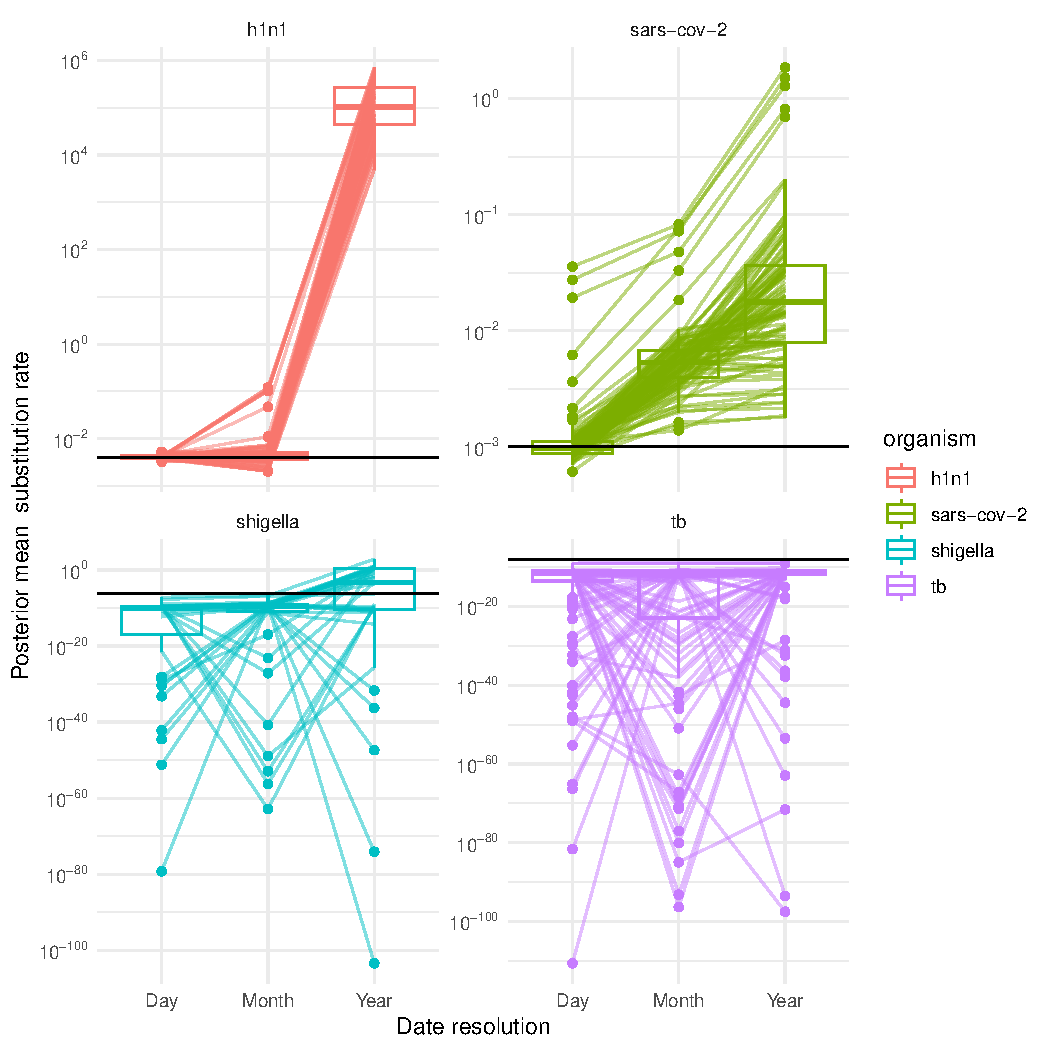
\includegraphics{sim_clock_trajectory.pdf}
    \caption{Mean posterior evolutionary rate for each simulation condition over decreasing date resolution. Lines connect individual simulated datasets across analyses with decreasing date resolution and horizontal black lines mark the true evolutionary rate. Mean posterior evolutionary rate increases where date roundeding clusters more divergent sequences, such as in the case of the viral datasets. The effect is less pronounced for the slower evolving simulation conditions - (\textit{S. sonnei} and \textit{M. tuberculosis}).}
    \label{fig:simClock}
\end{figure}

\begin{figure}
    \centering
    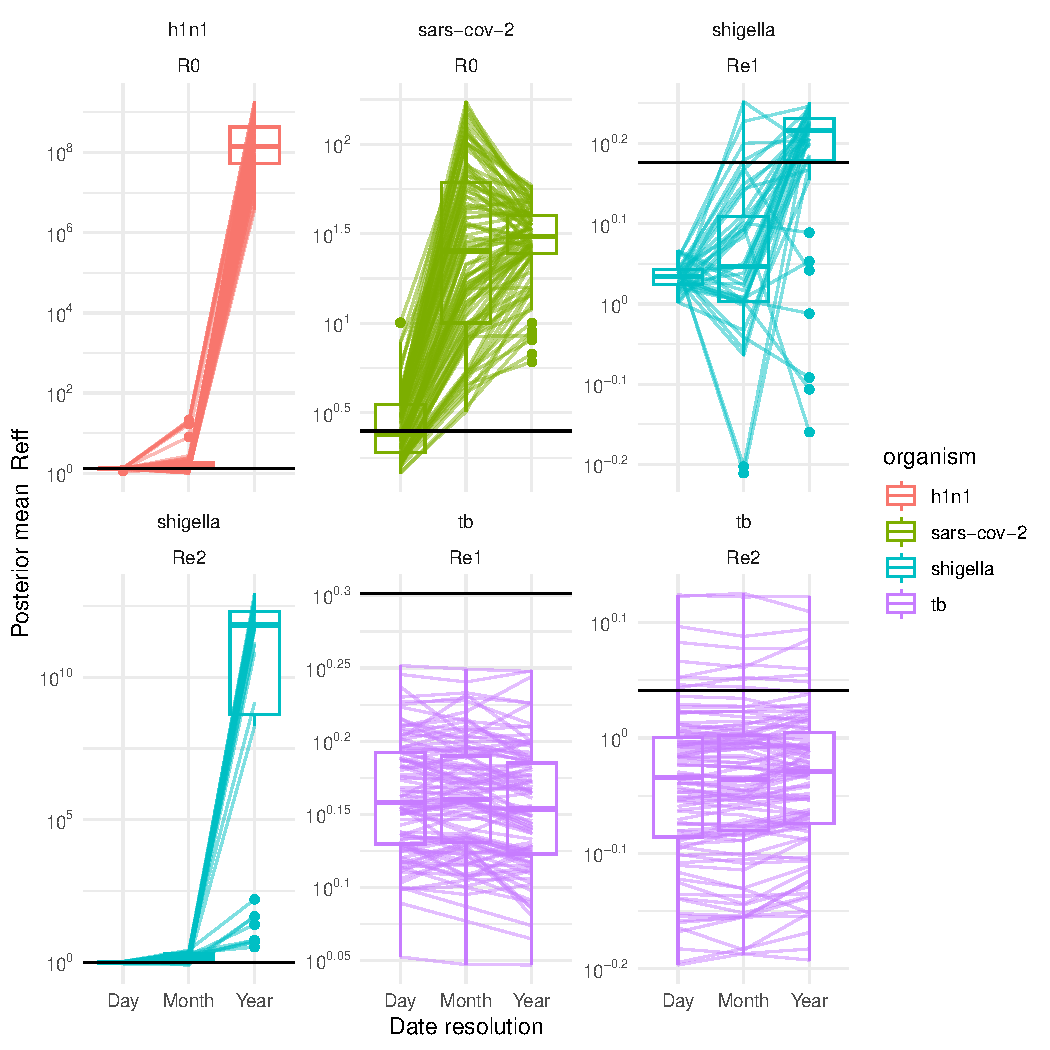
\includegraphics{sim_Re_trajectory.pdf}
    \caption{Bias in $R_0$ or $R_e$ over decreasing date resolution for simulated data. Lines connect posterior mean reproductive number for individual simulated datasets analysed under decreasing date resolution under each simulation condition. Horizontal black lines show the true value. In general, the reproductive number biases upwares with decreasing date resolution, with the most dimished effects where the date resolution is a smaller fraction of average time required for a mutation (\textit{S. sonnei} and \textit{M. tuberculosis}).}
    \label{fig:simR0}
\end{figure}

\subsection*{Empirical Results}
Broadly, analyses of the empirical datasets reproduce the trends of bias in reproductive number, substitution rate, and origin from the simulation study (figures \ref{fig:empR},\ref{fig:empClock}). That is, biases in the reproductive number increases with decreasing date resolution along with an increase in the substitution rate and corresponding decrease in the origin. There are a few exceptions to this trend that we consider below.

\subsubsection*{H1N1}
\subsubsection*{SARS-CoV-2}
The SARS-CoV-2 datasets behaves as expected from the simulation study, except for the origin under month resolution which is placed deeper in time. This is surprising given that the evolutionary rate is elevated at month resolution. (I need to check if this is a bug - are we rescaling with the true oldest sample or with the new date. Perhaps need to move these to a new plot.)
\subsubsection*{\textit{S. sonnei}}
\subsubsection*{\textit{M. tuberculosis}}

\begin{figure}[h!]
    \centering
    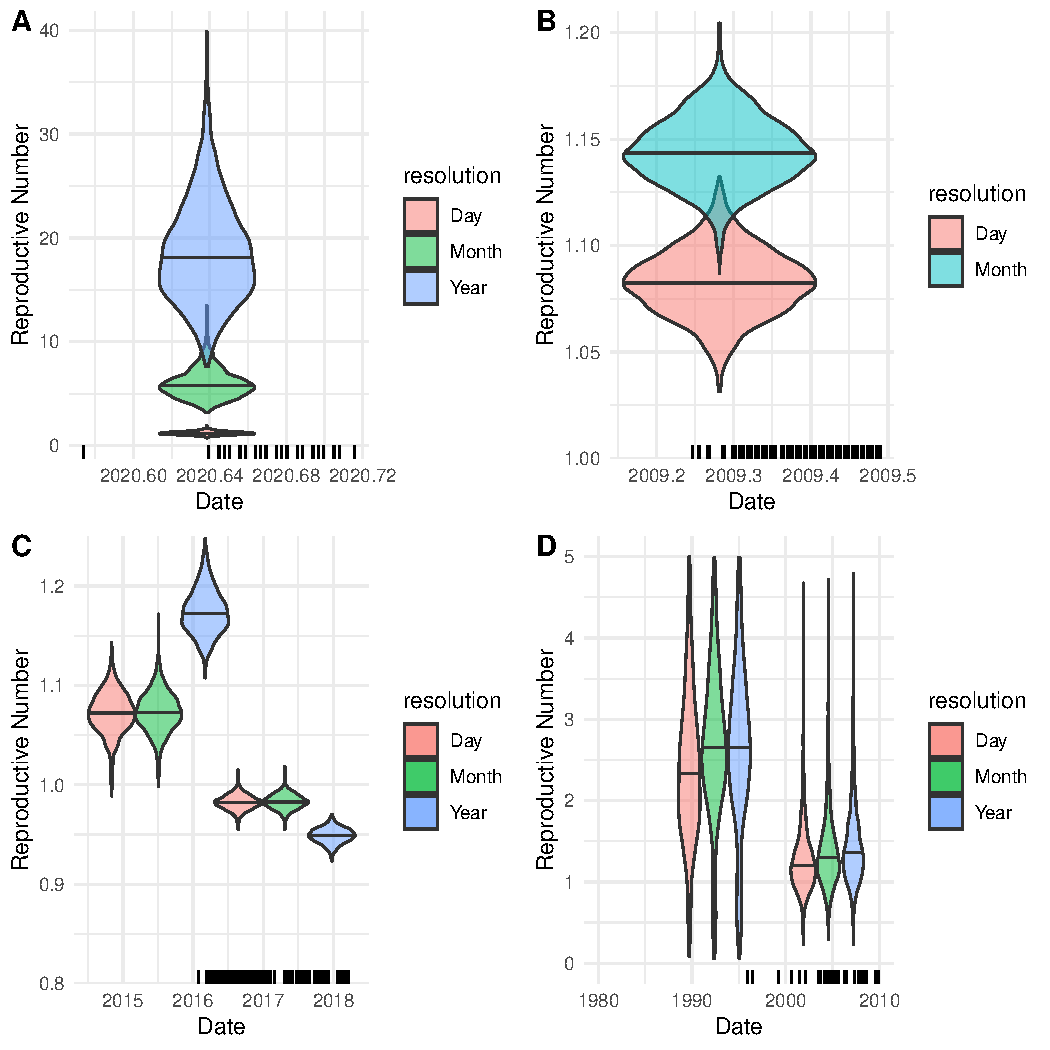
\includegraphics{empirical_plot.pdf}
    \caption{Posterior reproductive number and origin for each empirical dataset coloured by level of date resolution. Posterior origin times are represented as rescaled posterior frequencies along the Date axis and posterior reproductive numbers are given in violin plots on the vertical axis. For the H1N1 and SARS-CoV-2 datasets, posterior $R_0$ across date resolution is overlayed and overlaps minimally. For the \textit{S. sonnei} and \textit{M. tuberculosis}, posterior $R_{e_1}$ and $R_{e_2}$ (left to right) are displayed in adjacent groups. The change time between them is itself variable as half of the origin time. Samplng times are given as black mark son each date axis.}
    \label{fig:empR}
\end{figure}

\begin{figure}[h!]
    \centering
    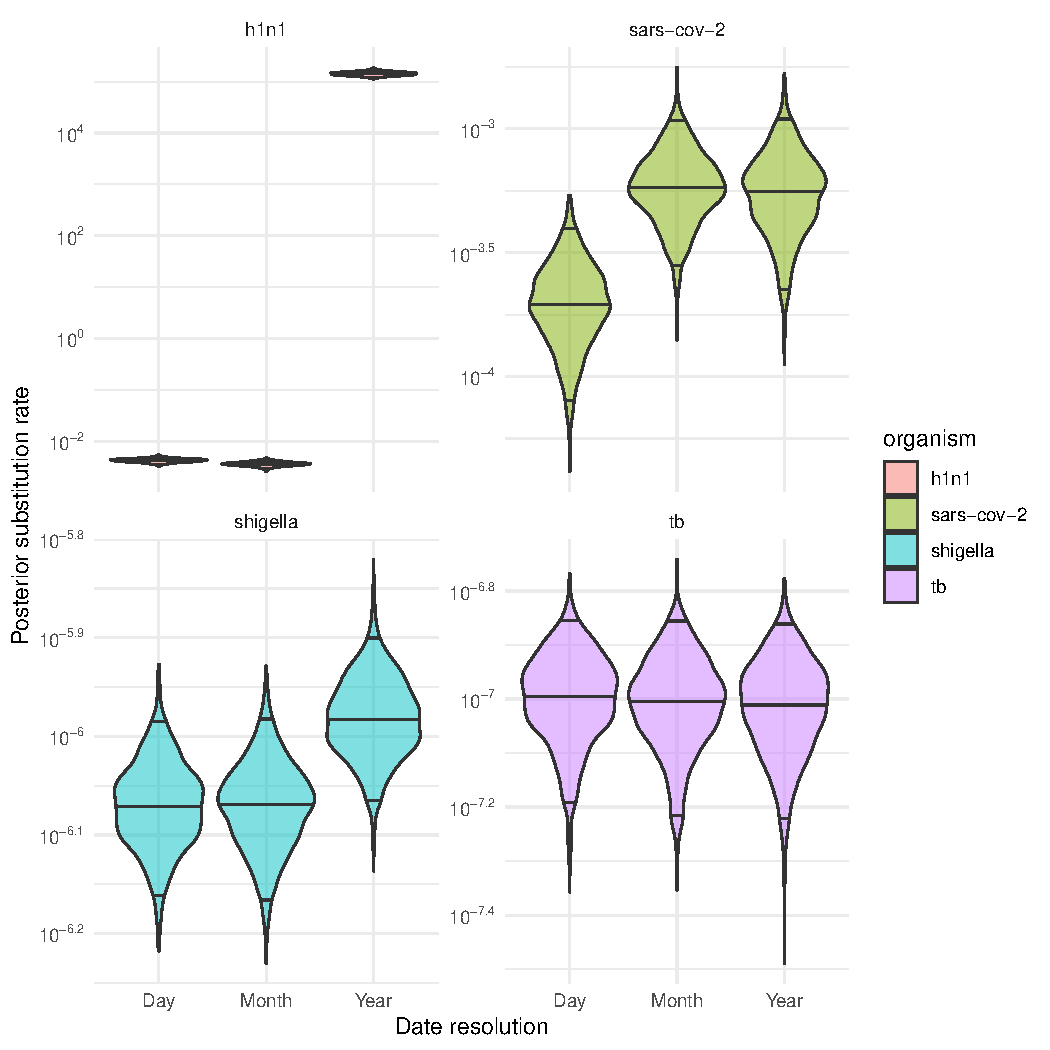
\includegraphics{empirical_clock_trajectory.pdf}
    \caption{Posterior substitution rate for each empirical dataset across analyses with decreasing date resolution.}
    \label{fig:empClock}
\end{figure}

\section*{Discussion}
\textbf{Brakdown of points to hit}
\begin{itemize}
    \item Bias doesn't move in one direction - depends on compression
    \item Why was each parameter biased the way it was?
    \item Overall, samples get clustered to the same time, but still have differences in sequence
    \item Suggests a higher mutation rate and transmission rate
    \item Hence spuriously large results for when we condense to year for H1N1
    \item Obviously, we would never rely on such results. For example, and $R_e$ of $10^8$ for H1N1 suggested the globe's population would be infected in one transmission event. Such is the blindness of our models. More tangibly though, we can always expect bias from what the full dates are suggesting, so the best thing to do is use the full date.
\end{itemize}
\subsection*{A simple solution}
The only information that matters, is the \emph{difference} between sequences and dates, rather than their absolute values. After all, our methods are comparative within a sample. Thus we can prioritise exact information and protect patient identity at the same time. We propose that authorities can provide dates that are all shifted in time by an unknown seed number, and reinterpret results by factoring this in. For example, if the sampling times of a dataset of 3 samples are (2000, 2001, 2002), then public health authorities may randomly draw a seed of 1000 with which to shift and dates and pass onto scientists: (2000, 2001, 2002) $\rightarrow$ (3000, 3001, 3002). Then results can be reinterpreted with regard to the random seed. If, for example the estimated time of onset was 3 years before the most recent sample, then those receiving the data will not be able to place this in time, while those on the data generation end can interpret this correctly (estimated time of onset = 2002-3 = 1999). In the same vein, transmission parameters such as $R_e$ can be understood to pertain to the true sampling time.

\end{spacing}

\bibliographystyle{natbib}
\bibliography{refs}

\subsection*{Supplementary Material}

\renewcommand{\thefigure}{S\arabic{figure}}
\setcounter{figure}{0}

\begin{table}[h!]
    \centering
    \caption{Substitution rates and genome length for sequence simulation.}
    \begin{tabular}{l|c|l|r}
    \hline
    Microbe                     &   Substitution Rate (subs/site/yr) & Genome Length & Subs/Genome/Time  \\
    \hline
    H1N1                        & $4\times10^{-3}$ & 13158 & 52.632\\
    SARS-CoV-2                  & $1\times10^{-3}$ & 29903 & 29.903\\
    \textit{S. sonnei}    & $6\times10^{-7}$ & 4825265  & 2.895\\
    \textit{M. tuberculosis}    &   $1\times10^{-8}$ & 4300000 & 0.043\\
    \hline
    \end{tabular}
    \label{tab:seq_parms}
\end{table}

\begin{figure}[h!]
    \centering
    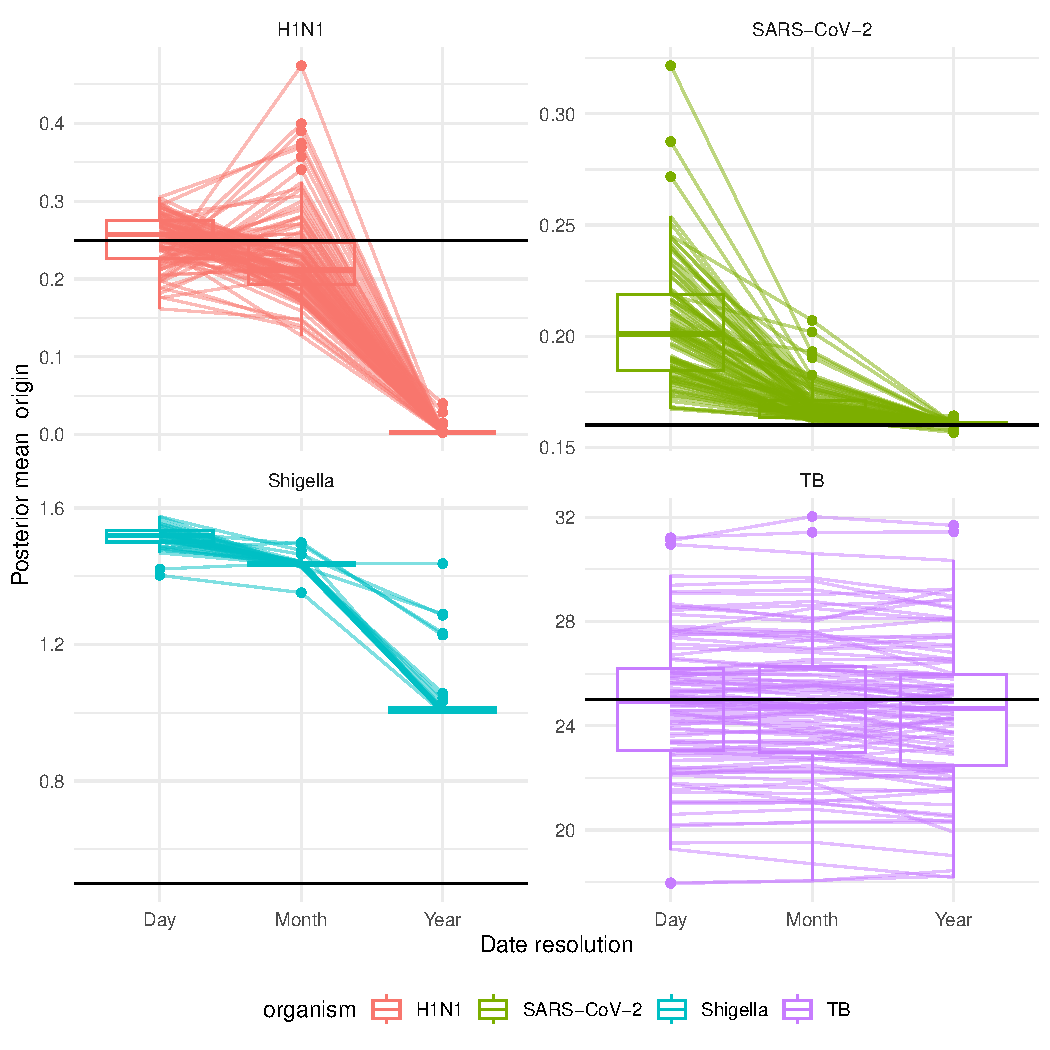
\includegraphics{sim_origin_trajectory.pdf}
    \caption{Meas posterior origin for each simulation condition over decreasing date resolution. Lines connect individual simulated datasets across analyses with decreasing date resolution and horizontal black lines mark the true evolutionary rate. Mean posterior origin decreases  where date roundeding clusters more divergent sequences, such as in the case of the viral datasets. The effect is less pronounced for the slower evolving simulation conditions - (\textit{S. sonnei} and \textit{M. tuberculosis}).}
    \label{fig:simOrigin}
\end{figure}

\end{document}